\chapter{Appetizers and Salads}

\section{Wedding Brunch Gazpacho\index{appetizers and salads!gazpacho}}

\textit{This gazpacho recipe comes by way of Jen Tidy.  
We were first introduced 
to it during the ``day
after'' wedding brunch.  The amounts of ingredients are variable, so add to your
personal taste preferences.} 
\begin{ingredients}
celery \\
peeled and seeded cucumbers \\
scallions and/or onions \\
red and green peppers \\
minced garlic \\
$\sim 6$ tomatoes (canned are O.K.) \\
$\sim 1/2$ cup of red wine vinegar \\
$\sim 1/2$ cup of olive oil \\
1--1\,1/2 cups tomato juice or V8 \\
lemon juice \\
black pepper \\
tabasco or cayenne pepper \\
fresh cilantro
\end{ingredients}
Chop the celery, cucumbers onion, peppers, tomatoes, and garlic to a
consistency that you find happy.  A food processor may be used for ``soupy''
consistency.  Mix the red wine vinegar and olive oil (these should be in equal
amounts).  To this add the tomato juice (V8).  Add lemon juice, black pepper,
tabasco, and fresh cilantro.  Combine veggies and liquid ingredients in a glass
pitcher or other asthetically pleasing container.  Chill for several hours or
overnight.  Serve with crunchy bread and a lightish red wine.

\section{Frog Mustard Salad Dressing\index{appetizers and salads!dressings}}

\textit{This is a quick preparation dressing 
that can be prepared in about 10 minutes.  It makes 8--10 servings}.
\begin{ingredients}
1/2 cup dijon mustard \\
2 Tbsp.  red wine vinegar \\
1/4 tsp. salt \\
3/4 tsp. pepper \\
1 cup corn oil (or olive)
\end{ingredients}
The crouton ingredients are:
\begin{ingredients}
4 slices fine textured white bread \\
4 Tbsp.  butter \\
1 tsp. dried thyme \\
1/8 tsp. salt \\
dash of pepper \\
2 tsp. minced parsley
\end{ingredients}
\begin{wrapfigure}{r}{4in}
\centerline{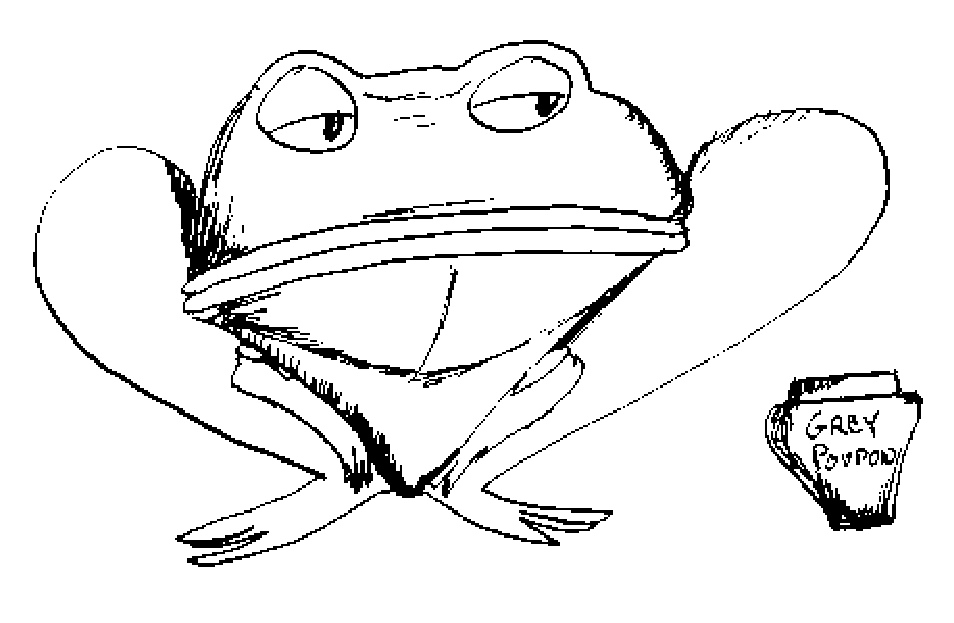
\includegraphics[width=3.8in,clip]{frog.ps}}
\end{wrapfigure}
To make the salad dressing wisk the mustard, vinegar, salt and pepper in a small
bowl.  Gradually add oil.

To make the croutons preheat the oven to \oven{350}.  Trim crusts (if desired)
and cut slices into 1/2$''$ cubes.  Spread single layer on tray, bake for 10--15
minutes until dry and lightly brown.  Heat butter in a skillet.  Add croutons and
remaining ingredients and toss well.  Saut\'{e} 1--2 minutes over medium heat and
cool.  Kate says that good salad stuffs are greenleaf or romaine lettuce with
spinach.  Add tomatoes, cucumber, and other salad stuff as your heart desires. 
Another yummy thing is to add pieces of chicken\index{salads, chicken} ham, or 
turkey and other meats, which makes it taste almost like a bite-sized sandwich.

\section{Easiest Tomato Aspic\index{appetizers and salads!tomato aspic}}

\textit{We received this recipe from Grammie (Lil Johnson) and we must 
confess we had no idea what an `aspic' was!  For those not in the know,
its a tasty treat.} 
\begin{ingredients}
1 small pkg. lemon \corp{Jello}\\
1 cup boiling water \\
1 8 oz. can \corp{Hunt's} Tomato Sauce \\
1 tsp. horseradish \\
(1 tsp. lemon juice or vinegar optional)  \\
\end{ingredients}
Add the following if you desire.
\begin{ingredients}
cooked shrimp \\
crabmeat \\
chopped celery
hard cooked egg \\
asparagus \\
articoke hearts \\
avocado \\
\end{ingredients}
Pour 1 cup boiling water over \corp{Jello} and mix until smooth. Add 
tomato sauce, horseradish, and lemon juice or vinegar. 
To this you can add any of the optional ingredients. Grandaddy's (Don)
favorites are seafood and chopped celery. Place aspic into fridge 
and jell about 3 hours. 

\section{Meaty Cheese dip\index{sides!Meaty Cheese Dip}}

\textit{Just so you know, this dish isn't good for you. But it's so delicious,
we don't care. Kate got this recipe from} \corp{Southern Living}.
\textit{For you food snobs, don't be put off by the} \corp{Velveeta}. 
\textit{It provides a smoothness in this dish. Trust me, I usually avoid it!}
\begin{ingredients}
1 lb. ground turkey or beef\\
1/2 lb. hot bulk pork sausage\\
1 8 oz. jar medium heat salsa\\
1 (2lb.) loaf \corp{Velveeta} with jalapenos, cut into cubes
\end{ingredients}
Brown ground meat and sausage in large skillet, stirring so it crumbles. Add
salsa and cheese and cook over low heat until the cheese melts. Serve warm
with nacho or corn chips. Yum!

\section{Hot crab dip\index{sides!Hot crab dip}}

\textit{This is sooo good! Martha and Dodge submitted this. This is a dip they
should make more often. But ha ha, now we have the recipe!}
\begin{ingredients}
8 oz. cream cheese, softened\\
1/2 lb. seafood flakes (fake crab legs)\\
2 Tbsp. chopped onion\\
Worchestershire sauce
\end{ingredients}
Preheat oven to \oven{350}. Mix cream cheese. Slice and add ``crab.'' Next add
onion and Worchestershire sauce. Bake for 15-20 minutes, or when bubbly.

\section{Blue Cheese-Pecan Spread\index{sides!Blue Cheese-Pecan Spread}}

\textit{This is an easy and yummy appetizer submitted by Martha and Dodge.
We usually spoil our appetite for dinner
eating it with all kinds of crackers!}
\begin{ingredients}
1/2 cup pecan pieces\\
4-5 oz. cream cheese\\
At least 2 Tbsp.  blue cheese, gorgonzola, or Roquefort\\
1-2 Tbsp.  butter \\
Worchestershire sauce and/or hot pepper flakes, optional
\end{ingredients}
In food processor, process pecans until fine. Add cream cheese and blue cheese
in small chunks. Add more blue cheese if it doesn't taste like enough.
``Smooth'' out flavors with the butter, if necessary. Add hot stuff if desired.
Spoon into crock or pretty bowl and refrigerate until ready to serve. 
